% ------------------------------------------------------------------------
% file `main-bookexercise-6-exercise-body.tex'
%
%     exercise of type `bookexercise' with id `6'
%
% generated by the `exercise' environment of the
%   `xsim' package v0.21 (2022/02/12)
% from source `main' on 2026/10/23 on line 652
% ------------------------------------------------------------------------
1. 关于下图所示的无向图，下列说法错误的是\underline{\hspace{1cm}}
\begin{center}
    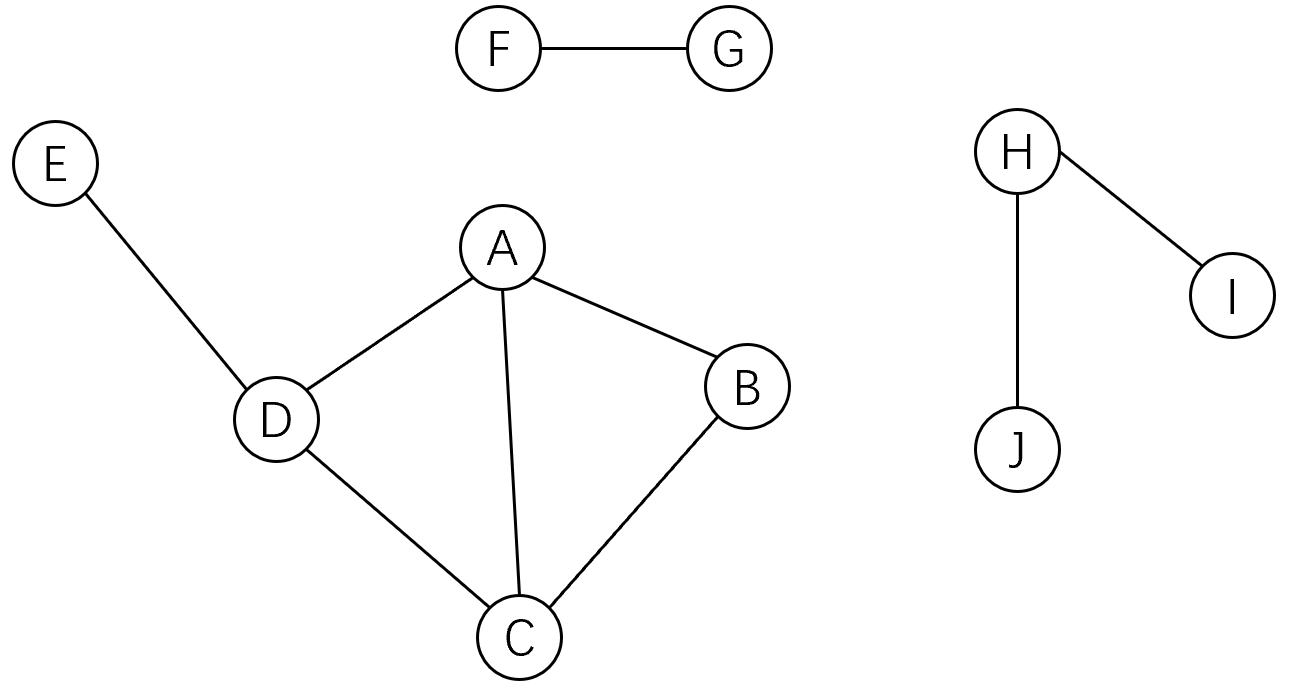
\includegraphics[width=0.48\textwidth]{assets/pics_and_ppts/ch5/习题01，图的基本概念.png}
\end{center}

\noindent A. 顶点A的度为3\\
B. 顶点A与顶点E是不连通的\\
C. 该图有3个连通分量\\
D. 对于顶点H所在的连通分量，若以H为起点，其深度优先搜索序列可以是\{H, I, J\}\\

2. 关于下图所示的有向图$G$以及其三个子图$G_1$, $G_2$, $G_3$，下列说法错误的是\underline{\hspace{1cm}}

\begin{center}
    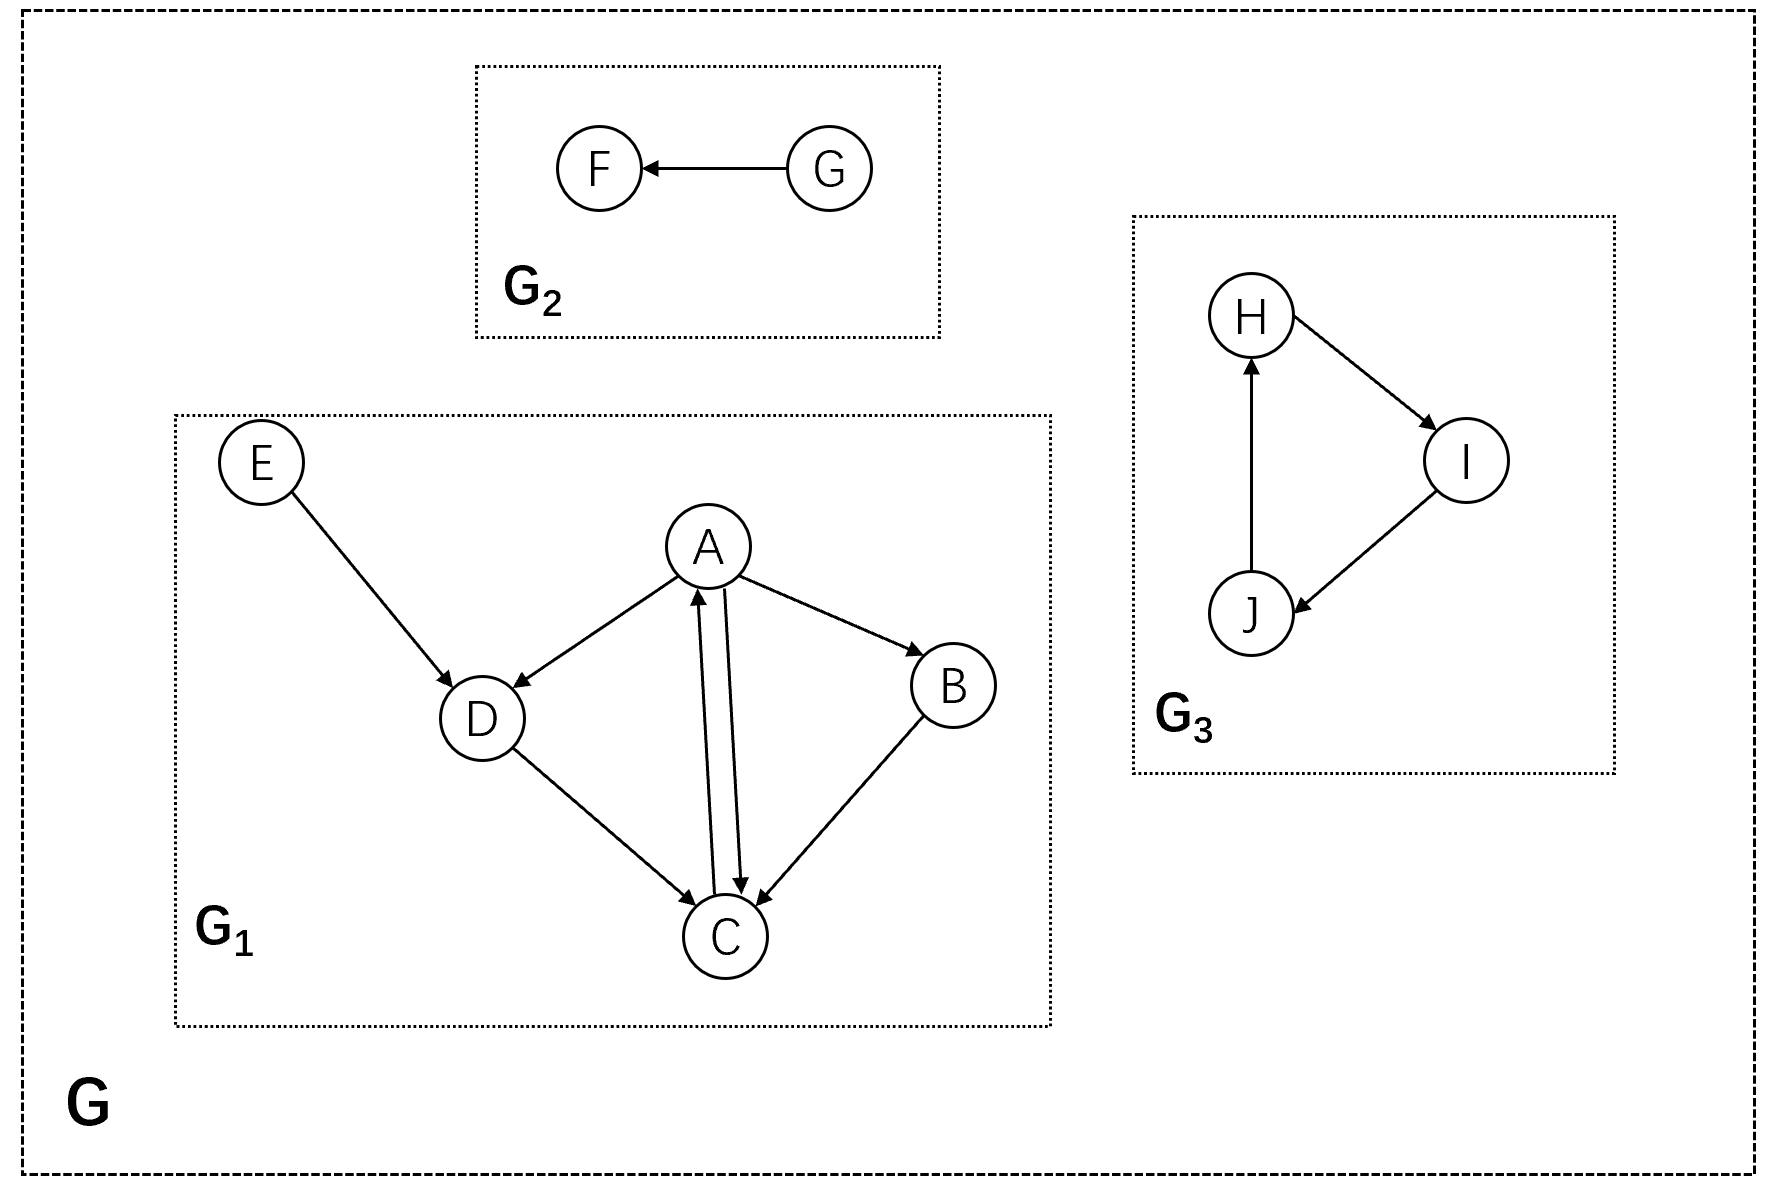
\includegraphics[width=0.72\textwidth]{assets/pics_and_ppts/ch5/习题02，图的基本概念.png}
\end{center}

\noindent A. 三个子图$G_1$, $G_2$, $G_3$中，仅$G_3$是强连通的\\
B. 图G的强连通分量数大于3\\
C. 顶点A的出度为3\\
D. 顶点F的出度为1\\

3. （某年408真题）下列关于无向连通图特性的叙述中，正确的是\underline{\hspace{1cm}}。

\(\mathrm{I}\). 所有顶点的度之和为偶数。

\(\mathrm{II}\). 边数大于顶点个数减 1。

\(\mathrm{III}\). 至少有一个顶点的度为 1。\\
A. 只有 \(\mathrm{I}\) \\
B. 只有 \(\mathrm{II}\) \\
C. \(\mathrm{I}\) 和 \(\mathrm{II}\) \\
D. \(\mathrm{I}\) 和 \(\mathrm{III}\) \\

4. 思考：有N个顶点的无向图，至多有多少条边？（不允许存在自环和重复边）。\\

5. 思考：有N个顶点的无向图，要保证它是连通图，至少要有多少条边？\\

6. 若无向图$G=(V, E)$有7个顶点，无边。现在要向图$G$中添加若干条边。请问，要保证无论怎样添加，添加$N$条边后图一定是连通的，则$N$最小是\underline{\hspace{1cm}}\\[0.5em]
\begin{tabular}{llll}
    A. 6 & B. 15 & C. 16 & D. 21
\end{tabular}

\vspace{\baselineskip}

7. 设某无向图的邻接矩阵A如下所示，若0表示边不存在，则各顶点的度依次是\underline{\hspace{1cm}}\\
\[
A =
\begin{bmatrix}
0 & 1 & 0 & 1 \\
1 & 0 & 1 & 1 \\
0 & 1 & 0 & 0 \\
1 & 1 & 0 & 0
\end{bmatrix}
\]

\begin{tabular}{llll}
    A. 2,3,1,2 & B. 4,6,2,4 & C. 0,1,2,3 & D. 999,1000,1001,7820
\end{tabular}

\vspace{\baselineskip}

8. 若上题的矩阵A表示的是某有向图的邻接矩阵，则各顶点的度依次是\underline{\hspace{1cm}}

提示：有向图中顶点的度定义为该顶点的入度和出度之和。\\
\begin{tabular}{llll}
    A. 2,3,1,2 & B. 4,6,2,4 & C. 0,1,2,3 & D. 999,1000,1001,7820
\end{tabular}

\vspace{\baselineskip}

9.


